\documentclass[a4paper, 11pt, twoside]{article}
\usepackage{preamble}

\usepackage{subfiles}

\title{\Title}
\author{\Author}
\date{\today}

\addbibresource{ref.bib}

\begin{document}
  \begin{titlepage}
    \thispagestyle{empty}
    \begin{center}
      \vspace*{1cm}

      \large
      \textsc{Travail d'Étude et de Recherche}
      \vspace{1.5cm}

      \huge\textbf{\Title}
      \vspace{2cm}

      \large
      Dorian Guillet
      \vspace{1cm}

      Encadré par Vincent Beffara.

      \vfill
      Mai 2025.
      \vspace{1cm}

      Institut Fourier -- M1 Mathématiques Générales
    \end{center}
  \end{titlepage}

  \newpage
  % \section*{Table des matières}
  \tableofcontents
  \thispagestyle{empty}

  \newpage
  \setcounter{page}{1}
  % \thispagestyle{empty}

  \addcontentsline{toc}{section}{Introduction}
  \thispagestyle{plain}
  \section*{Introduction}
    \subfile{sections/intro.tex}

  \newpage
  \section{Théorie des Types}
    \subsection{Introduction}
      \subfile{sections/type_theory/intro.tex}

    \subsection{Règles structurelles}
      \subfile{sections/type_theory/structural.tex}

    \subsection{Construction de types}
      \subfile{sections/type_theory/construction.tex}

    \subsection{Correspondance preuves -- programmes}
      \subfile{sections/type_theory/curry_howard.tex}

  \newpage
  \section{Formalisation du théorème de Bowen en Lean}
    \subfile{sections/lean/lean.tex}

  \newpage
  \section{Topologie des espaces ultramétriques}
    \subfile{sections/ultra/ultra.tex}

  \newpage
  \nocite{*}
  \thispagestyle{plain}
  \printbibliography[heading=bibintoc, title={Bibliographie}]

  \clearpage
  \addcontentsline{toc}{section}{Annexe}
  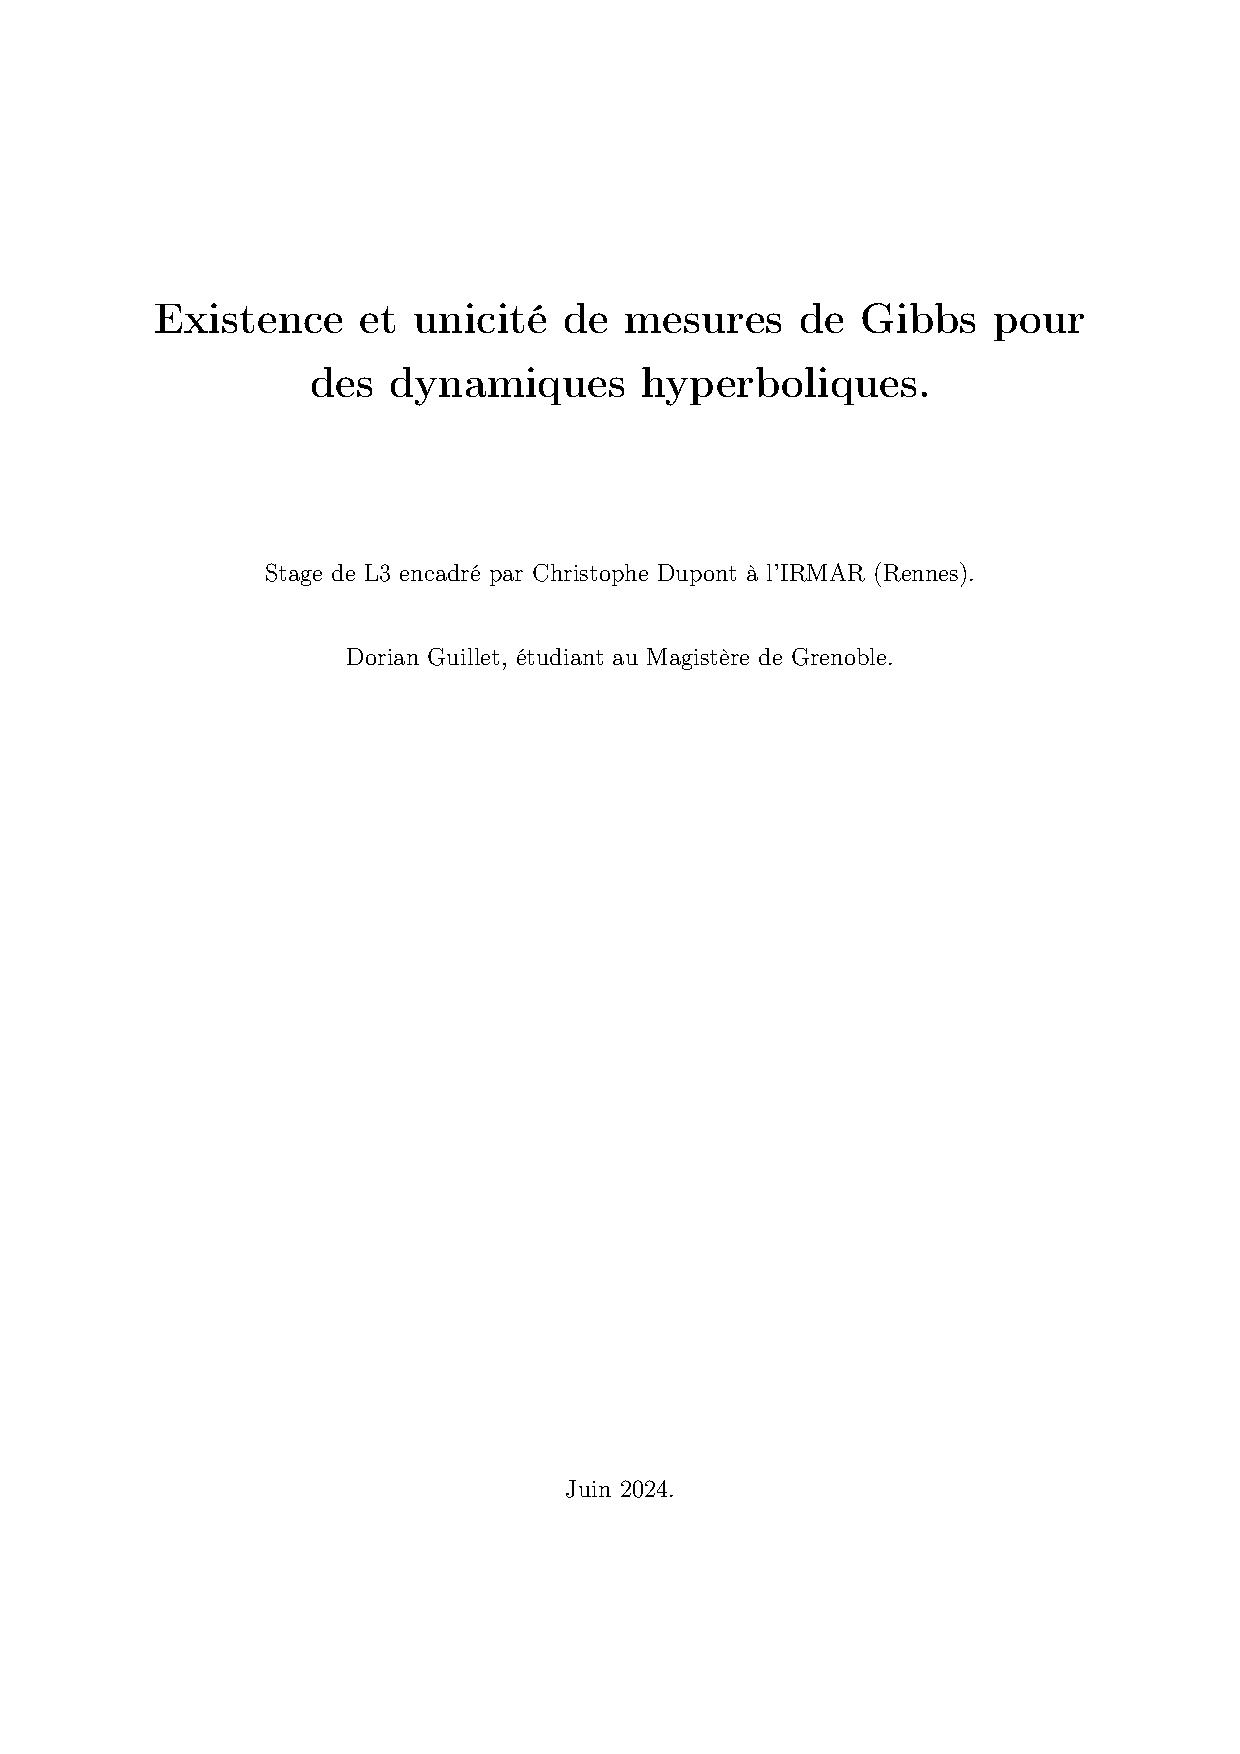
\includepdf[pages=-]{assets/stage.pdf}
  \addcontentsline{toc}{section}{Annexe4}

    % NOTE : https://lean-lang.org/theorem_proving_in_lean4/axioms_and_computation.html
\end{document}
